% SPDX-License-Identifier: Apache-2.0
% Compile with XeLaTeX, twice. The companion contains all referenced figures.
\documentclass[11pt,letterpaper]{article}
\usepackage[margin=0.82in,headheight=15pt,footskip=28pt]{geometry}
\usepackage{fontspec}
\setmainfont{NimbusRoman-Regular.otf}[BoldFont=NimbusRoman-Bold.otf,ItalicFont=NimbusRoman-Italic.otf,BoldItalicFont=NimbusRoman-BoldItalic.otf]
\setsansfont{NimbusSans-Regular.otf}[BoldFont=NimbusSans-Bold.otf,ItalicFont=NimbusSans-Italic.otf,BoldItalicFont=NimbusSans-BoldItalic.otf]
\setmonofont[Scale=0.80]{DejaVu Sans Mono}
\usepackage{amsmath,amssymb,mathtools}
\usepackage{microtype,graphicx,booktabs,tabularx,longtable,array,multirow}
\usepackage[table]{xcolor}
\usepackage{tikz}
\usetikzlibrary{arrows.meta,positioning,calc,shapes.geometric}
\usepackage{enumitem,titlesec,fancyhdr,caption,float,placeins}
\usepackage[most]{tcolorbox}
\usepackage{listings}
\usepackage{xurl}
\usepackage{hyperref}
\definecolor{Deep}{HTML}{211039}
\definecolor{Purple}{HTML}{6336A5}
\definecolor{Violet}{HTML}{9E76E9}
\definecolor{Lavender}{HTML}{F2EDF9}
\definecolor{Ink}{HTML}{262331}
\definecolor{Muted}{HTML}{625B70}
\definecolor{Teal}{HTML}{087E83}
\definecolor{Amber}{HTML}{91630C}
\definecolor{Rule}{HTML}{DDD4E9}
\hypersetup{colorlinks=true,linkcolor=Purple,urlcolor=Purple,citecolor=Purple,
 pdftitle={AGI ALPHA FLYWHEEL: Build the Next Advantage},
 pdfauthor={Vincent Boucher - MONTREAL.AI},
 pdfsubject={NADV-2026-01: executable capability construction, fresh work, and complete-cost succession},
 pdfkeywords={AGI ALPHA, SUCCESSOR Omega, program synthesis, productive capability, unit economics, reproducibility}}
\urlstyle{same}
\color{Ink}
\setlength{\parindent}{0pt}
\setlength{\parskip}{5.5pt plus 1pt minus 1pt}
\setlength{\emergencystretch}{3em}
\setcounter{tocdepth}{1}
\renewcommand{\topfraction}{0.94}
\renewcommand{\textfraction}{0.06}
\renewcommand{\floatpagefraction}{0.80}
\makeatletter
\setlength{\@fptop}{0pt}
\setlength{\@fpsep}{20pt}
\setlength{\@fpbot}{0pt plus 1fil}
\makeatother
\linespread{1.045}
\titleformat{\section}{\Large\sffamily\bfseries\color{Deep}}{\thesection}{0.6em}{}
\titleformat{\subsection}{\large\sffamily\bfseries\color{Purple}}{\thesubsection}{0.6em}{}
\titleformat{\subsubsection}{\normalsize\sffamily\bfseries\color{Deep}}{}{0pt}{}
\titlespacing*{\section}{0pt}{18pt}{8pt}
\titlespacing*{\subsection}{0pt}{12pt}{5pt}
\setlist{leftmargin=1.4em,itemsep=2pt,topsep=4pt,parsep=0pt}
\captionsetup{font=small,labelfont={bf,sf},textfont=normalfont,skip=7pt}
\newcolumntype{Y}{>{\raggedright\arraybackslash}X}
\newcolumntype{P}[1]{>{\raggedright\arraybackslash}p{#1}}
\newcommand{\status}[1]{{\sffamily\bfseries\small #1}}
\newcommand{\usd}[1]{\$#1}
\newcommand{\code}[1]{\texttt{\small #1}}
\newtcolorbox{evidencebox}[1][]{enhanced,colback=Lavender,colframe=Rule,
 boxrule=0.5pt,arc=3pt,left=11pt,right=11pt,top=9pt,bottom=9pt,#1}
\newtcolorbox{holdbox}[1][]{enhanced,colback=white,colframe=Amber,
 boxrule=0.8pt,arc=2pt,left=10pt,right=10pt,top=8pt,bottom=8pt,#1}
\pagestyle{fancy}
\fancyhf{}
\fancyhead[L]{\sffamily\small\color{Muted}AGI ALPHA FLYWHEEL}
\fancyhead[R]{\sffamily\small\color{Muted}BUILD THE NEXT ADVANTAGE}
\fancyfoot[L]{\sffamily\scriptsize\color{Muted}NADV-2026-01 \quad | \quad Research edition \quad | \quad 25 October 2026}
\fancyfoot[R]{\sffamily\small\color{Purple}\thepage}
\renewcommand{\headrulewidth}{0.3pt}
\renewcommand{\footrulewidth}{0pt}
\lstset{basicstyle=\ttfamily\scriptsize,breaklines=true,columns=fullflexible,
 backgroundcolor=\color{Lavender},frame=single,rulecolor=\color{Rule},
 xleftmargin=5pt,xrightmargin=5pt,framesep=6pt,showstringspaces=false}

\begin{document}
\begin{titlepage}
\pagecolor{Deep}\color{white}
\begin{tikzpicture}[remember picture,overlay]
 \fill[Purple,opacity=.25] ($(current page.north east)+(-1,-1)$) circle (5.4cm);
 \draw[Violet,opacity=.35,line width=.7pt] ($(current page.center)+(3.3,1.8)$) circle (5.0cm);
 \draw[Violet,opacity=.22,line width=.7pt] ($(current page.center)+(3.3,1.8)$) circle (6.3cm);
 \draw[Violet,opacity=.14,line width=.7pt] ($(current page.center)+(3.3,1.8)$) circle (7.6cm);
 \foreach \x/\y/\r in {1/2/.035,3/6/.025,7/4/.04,15/8/.025,16/19/.035,4/21/.02,18/24/.04,10/23/.025,12/16/.03,2/14/.025,18/13/.03,8/18/.025,15/3/.02,6/10/.025,19/6/.025,11/5/.02,2/25/.04,17/26/.02}
  \fill[white,opacity=.55] ($(current page.south west)+(\x,\y)$) circle (\r cm);
\end{tikzpicture}
\vspace*{0.45in}
{\sffamily\bfseries\fontsize{13}{17}\selectfont AGI ALPHA FLYWHEEL\hspace{0.5em}$\infty$\par}
\vspace{0.7in}
{\sffamily\bfseries\fontsize{38}{42}\selectfont BUILD THE\par NEXT ADVANTAGE\par}
\vspace{0.27in}
{\sffamily\fontsize{18}{23}\selectfont From Useful Work to\par Expanding Productive Capability\par}
\vspace{0.5in}
{\color{Violet}\rule{1.0in}{2pt}\par}
\vspace{0.18in}
\begin{minipage}{0.82\textwidth}
\large An executable study of example-driven capability construction,\newline
fresh work, complete costs and financeable succession.
\end{minipage}
\vfill
{\sffamily\bfseries\large SUCCESSOR $\Omega$ HARNESS\par}
\vspace{5pt}
{\sffamily ACTIVATE. EVOLVE. SCALE.\par}
\vspace{12pt}
{\small TRANSFORMATIONAL INTELLIGENCE $\infty$\par}
{\small Applicable \$AGIALPHA utility is documented by source and route.\par}
\vspace{0.4in}
{\sffamily\small Vincent Boucher\quad $\cdot$\quad MONTREAL.AI\par}
{\sffamily\small 25 October 2026\quad |\quad Study NADV-2026-01\par}
\vspace{0.2in}
{\footnotesize Local research executed. Monetary outcomes modeled.\newline
Persistent authenticated operation and real financial succession not run.\par}
\end{titlepage}
\nopagecolor\color{Ink}
\setcounter{page}{2}

{\sffamily\bfseries\color{Purple}\small ORIGINAL RESEARCH CONTRIBUTION}
\section*{Useful work can construct its next input capability.\newline The strongest incumbent still matters.}
\addcontentsline{toc}{section}{Research contribution and abstract}

\begin{abstract}
\noindent Can automated work support the construction of capabilities that make subsequent work more useful after their complete costs? We extend the existing AGI ALPHA Workbench and Autonomous Work Economy quote workflow with a finite, example-driven constructor of executable input adapters. The unchanged quote specialist already produces useful comparison packages, but requires canonical offers. The new constructor infers column and unit transformations from budgeted examples, qualifies each adapter on fresh work, and reuses admitted programs on later missions. An independently implemented Python verifier checks input semantics as well as the final cart and report. A frozen study covers 24 held-out schemas, 96 unique production missions, five methods and 24 separate boundary probes. Every method accepts 96/96 nominal missions; conventional active selection and a current LLM-assisted constructor each use 29 examples, versus 61 for ordinary reuse. A learned construction recipe also uses 29 and requires 31 development examples: improvement beyond the strong incumbent and sustained acceleration are not established. Complete-cost scenarios yield an active-method cost of \usd{1.211784} per accepted report in the base case, rising to \usd{15.863884} and \usd{650.040140} under lower utilization and shorter recovery horizons. These are modeled costs, not bills. Thirty nontransactional financing paths expose affordable, loss-making and delayed-payback cases for a hypothetical future capability. Actual collections and available earned surplus remain unknown. The contribution is an inspectable, source-bound construction-to-delivery loop with explicit technical qualification and economic non-promotion, rather than a claim of autonomous algorithmic invention or self-financing operation.
\end{abstract}

\begin{evidencebox}
\begin{tabularx}{\linewidth}{@{}P{0.18\linewidth}Y@{}}
\textbf{New capability} & 24 example-derived programs prepare previously unsupported raw-table inputs for the existing quote workflow. Each is qualified before three subsequent fresh reuses.\\[4pt]
\textbf{Strong comparison} & Active selection: 29 examples. Ordinary cached scripts: 61. Learned recipe: 29 plus 31 training examples. Current LLM-assisted constructor: 29; full model cost unknown.\\[4pt]
\textbf{Economic decision} & Keep the active specialist. Hold the extra learned recipe. Human-work savings remain duration thresholds; future financing remains simulation.\\
\end{tabularx}
\end{evidencebox}

\textbf{Scope of originality.} We contribute the AGI ALPHA-specific preparation contract, executable construction and qualification mechanism, source-bound evidence chain, and separated complete-cost admission experiment. Programming by example and active example selection are established ideas \cite{gulwani}. We do not claim their invention, a new quote-optimization algorithm, a superior general LLM, or a demonstrated recursively improving enterprise.

\clearpage
\tableofcontents
\vspace{12pt}
\begin{holdbox}
\textbf{Reading the evidence.} ``Accepted'' means that the complete synthetic research deliverable passed the declared independent verifier. It does not mean customer acceptance, production authorization or payment. ``Constructed'' means that a program was derived by the declared constructor from allowed examples. ``Modeled'' and ``simulated'' monetary quantities never become observed receipts.
\end{holdbox}
\clearpage

\section{Research question and immediate customer value}

The AGI ALPHA FLYWHEEL asks whether useful automated work can create resources for capabilities that make subsequent work more valuable, less costly or newly possible. A stronger hypothesis is that a retained capability improves the construction of the next capability. Both hypotheses need a complete causal record: useful output, an observed limitation, actual construction, fresh qualification, later reuse, costs and an affordable next decision. A favorable description of an existing solver does not supply this record.

The present offering is a bounded quote-comparison service. A customer supplies item quantities, supplier offers, pack sizes and prices, explicit exchange rates, shipping charges and a deadline. The service returns a recommended purchase basket, a readable report, an analysis record explaining exclusions and exact costs, and evidence linking the inputs to the calculation. It could replace the clerical preparation, arithmetic, comparison and report assembly in a competent human's quotation worksheet. It does not negotiate, certify suppliers, infer unstated commercial terms, procure goods or authorize payment. Equivalent human work must have the same deliverable and acceptance standard; comparisons with an entire procurement function would overstate replacement.

The existing service is useful when offers already have its canonical fields. Its unresolved preparation boundary is practical: supplier tables differ in column identity, units and money notation. The inspected TRANSFORMATIONAL INTELLIGENCE guide compares same-named columns, and the AWE quote adapter expects normalized offer objects \cite{alpha,awe}. We therefore select schema preparation as the next capability. We retain the established quote specialist and its existing delivery runtime. A new domain or a replacement optimizer would add little evidence about this actual bottleneck.

\subsection{Three separate estimands}

\textbf{A. Human-work economics} asks whether the delivered package can cost less than equivalent competent work without AI. Because matched human duration is unavailable, we compute explicit break-even durations from sourced labor rates and stated delivery assumptions. We do not invent a human completion time.

\textbf{B. Incremental Flywheel benefit} asks whether retained executable capability improves fresh production beyond ordinary reuse, a competent builder and established specialist methods, after training, construction, failure and maintenance. A cached adapter can be useful even if a conventional active selector is the best way to construct it. Retention alone does not establish a distinctive Flywheel advantage.

\textbf{C. Financeable succession} asks whether available earned resources, after costs, obligations and reserves, can fund beneficial further construction within its useful life. Affordability and value are jointly necessary. A profitable hypothetical service does not prove that the proposed next capability works; a useful capability does not prove that cash is available when needed.

Our primary technical unit is a schema-level construction problem followed by four fresh missions. Our economic unit is an accepted complete report. Those units must not be conflated with a string-conversion kernel, an invoice, a model token or an assumed token-market return.

\section{Foundations and the limitation addressed}
\label{sec:lineage}

We inspected the four requested repositories, the coordination record in issue \#4850, source artifacts and earlier manuscripts. Table~\ref{tab:lineage} states what the prior work supports and what this edition adds. Original manuscripts, study outputs, URLs and source histories remain unchanged. Several source and software lanes remain unmerged; publication of a passive paper is distinct from software qualification \cite{coordination}.

\begin{table}[htbp]
\small
\caption{Evidence lineage \cite{work,construction,capital,economic,awe}. Counts are prior-edition findings, not replications by this study.}
\label{tab:lineage}
\begin{tabularx}{\textwidth}{@{}P{0.22\textwidth}YY@{}}
\toprule
Foundation & Established within its scope & Remaining limitation\\
\midrule
Economics of Autonomous Work & 36/36 fresh exact-reconciliation jobs; conditional labor thresholds. & Matched human duration and complete deployed cost unknown.\\[4pt]
Capability construction & 42/42 primary jobs; actual parent/child calls; specialist comparisons. & Repair loses on 12/12 fresh cases; three cycles admit no improvement. Evidence adapter was externally authored.\\[4pt]
Productive Capital Engine & 72 scoped results; assurance, planning and dossier connection; cash and resource checks. & Child fresh-change CPU 4.069055 s versus 4.032727 s for ordinary caching; improvement HOLD.\\[4pt]
Economic Engine & 144 financial paths separate collections, reserves, failed candidates and finite-life payback. & No primary path buys a new candidate or capacity; simulation does not construct a method.\\[4pt]
Autonomous Work Economy & 16 accepted packages and 8 intended refusals; separate quote transfer 8/8 for successor and MILP, 2/8 for initial capsule. & Capability templates and solver composition were authored in advance; canonical input preparation assumed.\\[4pt]
This edition & Example-derived input programs; first fresh qualification before reuse; full alternative and cost record. & Synthetic bounded domain; no superiority to active selection, measured customer savings or observed self-financing.\\
\bottomrule
\end{tabularx}
\end{table}

The source-assurance workflow remains an important commercial foundation: it checks approved public source identities, inventories discrepancies and produces actions and reports. It does not certify behavior or security. Its exact-key/hash incumbent remains appropriate. Its current improvements are safety engineering, not automatically autonomous invention. Likewise, planning capabilities and the earlier repair specialist provide real reusable components without establishing a superior learned builder \cite{construction,capital}.

We use the released Alpha \code{createWorkbench(adapters)} extension seam, the unchanged AWE quote normalization and supplier-subset solver, existing source/mission identities, pack integrity and unfunded Jobs compilation. We import the owner's exact \code{alpha-automated-costs/v1} and \code{alpha-shadow-ledger/v1} implementations. The new module is a bounded adapter and constructor; it is not another runtime, scheduler, accounting schema or publishing system.

The contribution therefore addresses a narrower and previously unresolved link: \emph{can evidence from a useful workflow produce a new executable preparation capability, be checked independently on fresh work, and be retained with a defensible economic decision?} It tests this link even when the next learned construction method deserves rejection.

\section{Useful deliverable and acceptance contract}
\label{sec:deliverable}

\subsection{What the user receives}

Each accepted pack contains five useful artifacts: \code{quote-report.md}, \code{recommended-cart.csv}, \code{quote-analysis.json}, \code{constructed-adapter.json} and \code{prepared-offers.json}. The first three come from the existing quote workflow; the last two expose how raw input became canonical offers. The Workbench supplies source and mission bindings, integrity digests, evaluation labels, a chronicle and seven unfunded Jobs drafts. Draft compilation does not submit jobs or move money.

For every requested item, the basket selects one eligible supplier offer and enough integral packs to cover demand. It includes the applicable rational exchange-rate conversion, exact declared rounding, supplier shipping charged once, and deadline exclusions. The independent oracle enumerates feasible carts using a separate Python implementation and verifies the optimum and declared constraints. Equal-cost alternative baskets are permitted if they satisfy the same exact acceptance standard. The service does not infer exchange rates or interpret open-ended free text.

The complete-output check also verifies every prepared offer against evaluator-owned canonical input, the CSV and report totals, and the analysis. This input check matters: two solvers that share the same incorrectly normalized input can agree perfectly and still deliver the wrong result. Workbench integrity inspection alone is insufficient to establish semantic correctness.

\subsection{Automated operating configuration and residual work}

The local configuration performs typed preparation, construction, planning through the existing adapter, execution, verification, artifact packaging and explicit refusal. It caches only a qualified program under the complete schema contract. A first fresh qualification failure prevents reuse; the expected answer is never fed back to repair a held-out program. Atomic journal writes preserve completed events, and bounded cancellation is available. The demonstration offers inspection, downloads and a restartable local run.

Correction is deliberately constrained. Unsupported or ambiguous input is refused with a reason; it is not silently coerced. A user or operator must resolve an unknown schema, provide a reviewed example, correct a missing exchange rate or repair a contradictory source record. The model charges example preparation, exceptions, retries, maintenance, setup and customer attention explicitly. Remote recovery, scheduled intake, network reconnect, browser-close persistence and clean installation on an approved execution profile were not run. Atomic local output is not evidence of those service properties.

\begin{evidencebox}
\textbf{Concrete example, not a sale.} H01 needs two selected worked examples to identify its adapter. Its first fresh synthetic basket totals 858,559 USD minor units; the next totals 2,824,085. Both complete packages pass the separate Python check. They are different purchase requests, so the difference in totals is not a saving. The reusable asset is the exact mapping and interpretation program, not either basket's answer.
\end{evidencebox}

\section{An executable construction loop}
\label{sec:method}

\subsection{Program space and declared permissions}

A schema task has 6--10 distinct headers and a pool of 16 unlabeled rows. It exposes an oracle for a reviewed row's six canonical values: item, vendor, pack units, pack price in minor units, currency and lead days. Each program assigns every canonical field a source column and one allowlisted operation. It is inert JSON interpreted by a finite grammar; no input-supplied source code is evaluated.

Text is trimmed without changing interior content. Currency is an explicit three-letter code. Pack counts accept integers, declared suffixes such as ``units'' or ``pièces'', or an \code{xN} prefix. Lead time accepts integers, declared day suffixes or weeks multiplied by seven. Prices accept bare nonnegative integer minor units, or nonnegative decimal point/comma notation with exactly two fractional digits. Only the decimal forms permit an optional leading \$ or euro symbol or a trailing three-letter currency code, never both; \$ must agree with USD and the euro symbol with EUR. Bounds, identity collisions and currency conflicts are checked. Thousands separators, approximate currency inference, arbitrary transformations and undeclared semantics are outside scope.

The researcher supplies this grammar, constructor, tools, budgets, acceptance standard and experimental infrastructure. The system chooses the mapping and operation for each actual schema from permitted evidence. No superior schema-specific mapping is manually inserted as a candidate. Constructed artifacts, alternatives eliminated, labels queried and failures are recorded. This is \emph{new executable construction within an authored grammar}; the quote solver is adoption and reuse; the Workbench seam is integration. None is presented as autonomous algorithmic invention.

For field $f$, let $V_f$ be the finite set of candidate column--operation pairs valid on the unlabeled pool. After querying row $i$ with canonical value $y_{if}$, the constructor updates
\begin{equation}
 V_f \leftarrow \{p\in V_f:p(x_i)=y_{if}\}.
\end{equation}
It emits a program only after at least one example and exactly one survivor for every field. Empty spaces, unresolved ambiguity, cancellation or exhausted budget produce refusal. The limits are eight labels and 200,000 candidate-evaluation operations per construction. Selection operations are separately counted and included in measured constructor CPU/wall time. Equal caps do not imply equal consumed resources.

\subsection{Ordinary and learned construction policies}

The ordinary builder queries rows in their declared order. Conventional active selection chooses an unqueried row maximizing normalized disagreement across fields. If $n_{fiv}$ candidates predict value $v$, its score is
\begin{equation}
 S(i;w)=\sum_f w_f\left(1-\frac{\sum_v n_{fiv}^{\,2}}{\max(1,|V_f|^2)}\right).
\label{eq:selection}
\end{equation}
The established active policy uses $w_f=1$. The experimental retained recipe measures unresolved alternatives after development examples, $d_f=\sum_{t,e}\max(0,|V_{f,t,e}|-1)$, and derives
\begin{equation}
 w_f=1+\operatorname{round}\left(7d_f/\max(1,\max_g d_g)\right).
\end{equation}
This one retained construction capability is then evaluated on unseen schema problems. Its weights are item 5, vendor 1, pack units 2, price 8, currency 1 and lead days 1. They are computed from traces rather than set after looking at held-out performance. The recipe is a hypothesis about better example selection; transfer and repayment are tested separately.

\subsection{From mission evidence to the next mission}

Figure~\ref{fig:loop} shows the execution and decision boundaries. The companion's connected replay first runs a canonical seed job through the unchanged adapter and verifies it. A raw-table request then encounters the actual preparation boundary (the existing workflow reports \code{OFFER\_LIMIT} without canonical offers). The study constructor derives H01's program, the first fresh mission qualifies it, the next reuses it, and the shared ledger records the unknown real financial position. This is a scripted, after-outcome replay connecting executed study cases, not an additional independent experiment or evidence of autonomous mission-family selection.

\begin{figure}[htbp]
\centering
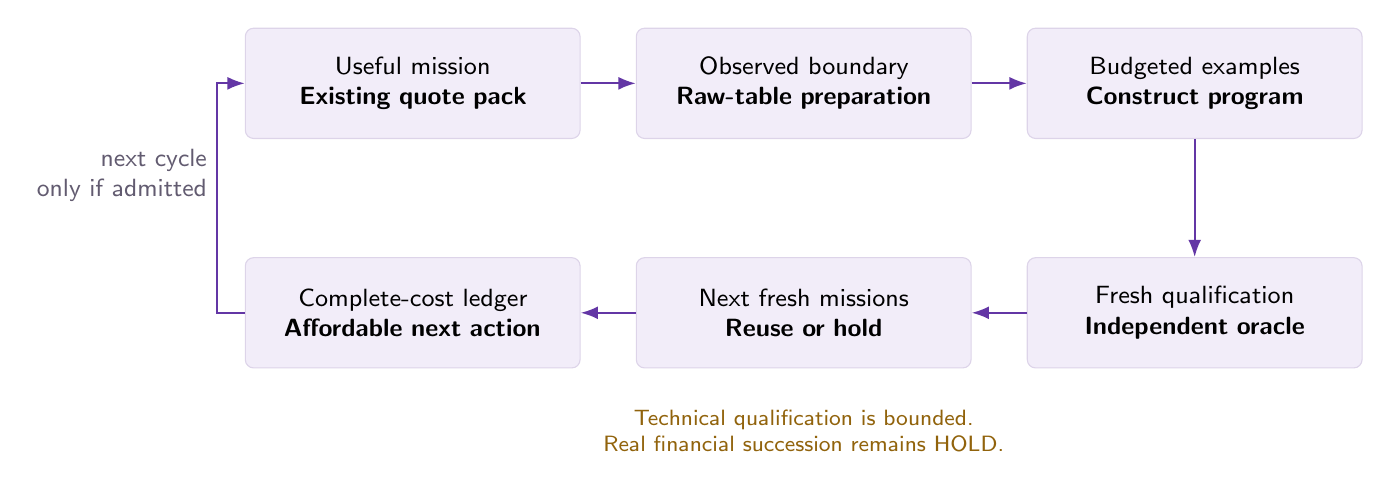
\begin{tikzpicture}[font=\small\sffamily,node distance=9mm and 7mm,
 box/.style={draw=Rule,fill=Lavender,rounded corners=3pt,align=center,text width=39mm,minimum height=14mm,inner sep=5pt},
 arrow/.style={-{Latex[length=2.2mm]},draw=Purple,line width=.8pt}]
\node[box] (work) {Useful mission\\\textbf{Existing quote pack}};
\node[box,right=of work] (evidence) {Observed boundary\\\textbf{Raw-table preparation}};
\node[box,right=of evidence] (construct) {Budgeted examples\\\textbf{Construct program}};
\node[box,below=15mm of construct] (verify) {Fresh qualification\\\textbf{Independent oracle}};
\node[box,left=of verify] (reuse) {Next fresh missions\\\textbf{Reuse or hold}};
\node[box,left=of reuse] (ledger) {Complete-cost ledger\\\textbf{Affordable next action}};
\draw[arrow] (work)--(evidence);\draw[arrow] (evidence)--(construct);
\draw[arrow] (construct)--(verify);\draw[arrow] (verify)--(reuse);
\draw[arrow] (reuse)--(ledger);
\draw[arrow] (ledger.west)--++(-.35,0)|-node[pos=.3,left,align=right,text=Muted]{next cycle\\only if admitted} (work.west);
\node[below=4mm of reuse,text=Amber,align=center,font=\footnotesize\sffamily] {Technical qualification is bounded.\\Real financial succession remains HOLD.};
\end{tikzpicture}
\caption{The executed connection. New scientific acceptance is separate from existing pack integrity. Hypothetical financing scenarios cannot clear the final real-money gate.}
\label{fig:loop}
\end{figure}

\begin{table}[htbp]
\small
\caption{The intended journey mapped to concrete actions and evidence. The execution order loops through useful work; names do not imply additional unexecuted reasoning modules.}
\begin{tabularx}{\textwidth}{@{}P{.17\textwidth}YY@{}}
\toprule Stage & Input, action and artifact & Measurable contribution\\\midrule
Identify & Supported quote input; select complete report contract; save seed input. & Defines the accepted useful unit.\\[3pt]
Out-Learn & Verified seed and failed raw-input attempt; record preparation boundary. & One observed contract limitation, not a benchmark victory.\\[3pt]
Out-Think & Boundary and permitted grammar; choose finite example-driven preparation. & Search limited to six fields, eight labels and explicit operations.\\[3pt]
Out-Design & Allowed examples; execute constructor; save program and elimination trace. & 24 programs per retained builder; observed acquisition cost.\\[3pt]
Out-Strategise & Frozen comparison and shared costs; keep active incumbent. & Extra learned recipe not economically promoted.\\[3pt]
Out-Execute & Fresh rows and program; run unchanged quote specialist; verify pack. & 96/96 accepted per method.\\[3pt]
Out-Evolve & Qualified program and ledger; reuse on next jobs; assess next action. & 72 subsequent reuses per caching method; real finance HOLD.\\
\bottomrule
\end{tabularx}
\end{table}

\section{Prospective evaluation and comparators}
\label{sec:design}

\subsection{Freeze, separation and independent verification}

Before confirmatory outcomes, the protocol freeze bound 371 files: the grammar, source modules, cost assumptions, input commitments, primary criteria, evaluator and sealed data. It was recorded at 21:02:05 UTC on 25 October 2026. The freeze identifier begins \code{d0d0f94598c86f3b}; the full identifier and file hashes are in the companion. The confirmation runner checks every frozen file before running. The LLM constructor has its own subsequent source/program freeze before any production evaluation.

Twelve development schemas cover plain minor-unit prices, suffix/dot notation and prefix/comma notation, four each. Twenty-four held-out schemas contain four instances of each of six families: the same three types plus weekly lead times, currency affixes and mixed alternative views. The last three are unseen structural compositions within the disclosed grammar, not arbitrary new language features. Header identities and exact configurations are disjoint. Four fresh production missions per held-out schema yield 96 unique jobs. All use synthetic, nonpersonal data; no market sampling is implied.

The builder sees the task's unlabeled example pool and only explicitly requested canonical labels. It does not receive production expected outputs. Evaluation ownership is separate within the collaborating research session. The Python verifier independently implements exact arithmetic and Cartesian cart search, checks normalized input truth, and imports neither the candidate nor the JavaScript quote solver. It was exercised on existing AWE cases and deliberately mutated outputs before freeze. This is implementation independence, not external institutional peer review or cryptographic isolation from the supervising agent.

The first fresh mission is the technical qualification trial. Only after its independent pass may the program be reused on the next three. Confirmation is frozen and nonadaptive: failures do not change the candidate. Every case remains in the denominator. An incorrect accepted output violates the primary safety criterion; refusals reduce delivered coverage. Twenty-four separate boundary probes test expected rejection, rather than being counted as useful deliveries.

\subsection{Five methods with legitimate improvement opportunities}

\begin{enumerate}
\item \textbf{Rebuild ablation.} The ordinary sequential constructor runs anew for every mission. This exposes construction repetition; it is not the strongest comparator.
\item \textbf{Ordinary reuse.} The same constructor uses schema-keyed reusable programs after qualification. This gives conventional caching and scripts their legitimate benefit.
\item \textbf{Retained construction recipe.} The same grammar, constructor and cache use the learned weights in Equation~\ref{eq:selection}. Development is charged.
\item \textbf{Active specialist.} Conventional maximum-disagreement selection has the same grammar, label cap, candidate cap and cache, without recipe training. This is the principal strong deterministic comparator.
\item \textbf{Current LLM agent with standard tools.} A separate clean-context assistant authors and runs a Python finite-grammar constructor using allowed public examples and a bounded oracle CLI. It may construct reusable capabilities and receives a grammar reviewer. Its programs are frozen before production feedback and delivered through the same runtime and verifier.
\end{enumerate}

The current LLM comparator is an actual same-session tool-assisted execution, not a hypothetical API agent or a static result attributed to a model. Its action log, source revisions, selected labels, programs, parser checks and recorded-label replay are retained. A limited incidental sibling-summary metadata exposure is disclosed; no production inputs, expected results or candidate implementation were opened before its freeze. Model inference time, provider token counts and billing are unexposed. Therefore it supports output and example-efficiency comparison but not a matched-dollar or externally blinded LLM benchmark. Its Python operation counters are also not a portable instruction-equivalent measure against JavaScript.

All methods use the same existing quote specialist downstream. A different optimizer would not resolve preparation and would confound this study. AWE already compared its quote method with conventional MILP \cite{awe}. Here the relevant established specialist is active example selection; we retain it when it wins.

\subsection{Primary outcomes and uncertainty}

Primary outcomes are accepted complete outputs, false acceptance, refusal and example acquisition. We also record constructions, hypothesis evaluations, selection operations, CPU/wall spans, artifact bytes, reuse and unknown monetary fields. All four deterministic arms are interleaved with rotating order. The LLM production evaluation follows its independent freeze and is not timing-interleaved with them.

The paired query analysis uses schemas as clusters, with all four missions linked. We resample four schemas within each of the six family strata, using 10,000 bootstrap draws and seed 20261025. The interval describes this generated workload, not market demand or universal schema performance. Tiny single-host CPU differences are descriptive; no service-pricing or general latency claim rests on them. Complete process CPU is unknown because Python startup/teardown CPU was not instrumented; complete verification wall time includes process launch.

\section{Results: useful construction, a strong tie, no acceleration}
\label{sec:results}

\begin{table}[htbp]
\small
\caption{All primary methods on the same 96 unique fresh jobs. Counts across columns are repeated evaluations, not independent customer jobs. Additional learned-recipe training is separate.}
\label{tab:results}
\begin{tabularx}{\textwidth}{@{}Yrrrrr@{}}
\toprule Method & Accepted & Builds & Labels & Extra training & False accepts\\\midrule
Rebuild & 96/96 & 96 & 244 & 0 & 0\\
Ordinary reuse & 96/96 & 24 & 61 & 0 & 0\\
Retained recipe & 96/96 & 24 & 29 & 31 & 0\\
Active specialist & 96/96 & 24 & 29 & 0 & 0\\
Current LLM-assisted & 96/96 & 24 & 29 & See text & 0\\
\bottomrule
\end{tabularx}
\vspace{4pt}
{\footnotesize The LLM constructor used 15 selected examples during its 12-schema public development run and validated all 192 public development labels. Its source-authoring/model cost is unknown; these counts do not make it cost-free.}
\end{table}

All 480 method--job evaluations pass on the 96 unique production missions. There are no nominal refusals or independently rejected outputs. Each caching method qualifies 24 programs and uses them on 72 subsequent jobs. The untouched canonical-input workflow has no raw-table adapter; the new programs expand the input forms it can deliver on. This establishes scoped input-capability construction, not a quality advantage over the capable alternatives, which also deliver all jobs.

The active policy uses 32 fewer examples than ordinary reuse, a 52.46\% reduction from 61. The retained policy makes the same reduction but also consumes 31 development examples. The paired retained-minus-ordinary difference is $-1.333$ examples per schema, with a stratified bootstrap 95\% interval $[-1.833,-0.833]$. Retained-minus-active is exactly zero on every schema and has interval $[0,0]$. The LLM-assisted constructor independently selects 29 examples, at most two per held-out schema, and produces programs whose recorded-label replay exactly matches its frozen results.

\begin{figure}[htbp]
\centering\includegraphics[width=\textwidth]{figures/capability_queries.pdf}
\caption{Example acquisition for useful programs. The extra learned-recipe training is visible. Conventional active selection matches both the retained recipe and the actual LLM-assisted constructor on production labels. The LLM's authoring and model billing remain unknown.}
\label{fig:queries}
\end{figure}

\begin{table}[htbp]
\small
\caption{Family-level acquisition totals. Each family has four held-out schemas and 16 fresh missions per method. All corresponding deliveries are accepted.}
\begin{tabularx}{\textwidth}{@{}Yrrr@{}}\toprule
Family & Ordinary reuse & Retained recipe & Active specialist\\\midrule
Plain minor units & 14 & 6 & 6\\
Suffix / decimal point & 12 & 6 & 6\\
Prefix / decimal comma & 4 & 4 & 4\\
Weekly lead times & 6 & 4 & 4\\
Affixed currency & 8 & 4 & 4\\
Mixed alternative views & 17 & 5 & 5\\\bottomrule
\end{tabularx}
\end{table}

\subsection{Resource record and meaningful failures}

The deterministic rebuild, ordinary, retained and active methods perform respectively 44,420, 11,105, 10,866 and 10,866 candidate evaluations. Retained and active each record 9,053 selection operations. Constructor CPU totals are 91.378, 19.408, 23.021 and 25.772 ms. Whole recorded mission wall totals, including verification and packaging, are approximately 5.857, 5.785, 5.785 and 5.881 seconds over 96 reports. These small one-run differences do not establish a general speed ranking.

The LLM-authored CLI records 38,591 conservative parse/comparison budget units, 37,272 selection operations and 766.133 ms of per-schema constructor CPU. Its combined recorded construction-and-delivery wall time is about 7.023 seconds, including 0.763 seconds of construction and 6.259 seconds of delivery, verification and packaging. These omit model inference and interactive authoring, and its counters differ in granularity. We therefore make no inference that either language, constructor or LLM is economically faster from these figures.

All 24 unique boundary probes reject as required across the three deterministic selection policies, yielding 72 repeated checks. The six groups cover indistinguishable columns, conflicting currency affixes, identity collisions after normalization, malformed or out-of-bounds values, schema drift, and unsupported semantic identities or exchange rates. Four ambiguous cases consume the eight-label budget and refuse. The separate LLM constructor was not evaluated on those four construction-ambiguity probes; the 72 checks must not be attributed to all five constructors. Such refusals are correct behavior, not successful useful work or improved productive capability. A separate control suite checks budget exhaustion, cancellation and literal grammar behavior.

No nominal candidate failed after freeze, and none is omitted. Pre-freeze development corrections, all three development executions, source snapshots and failed checks remain in the package. The three executions contain 93 query calls but only one 31-example training episode; they are not three independent gains. Reporting amendments preserve the initial unstratified bootstrap output and the auxiliary CPU report that omitted packaging. Corrected reporting uses the prespecified family strata and all recorded CPU spans. Neither correction changes candidate source, labels, accepted outputs, cost tiers or financing decisions.

\subsection{What improved, and what did not}

\textbf{Better task execution is supported within scope.} A qualified retained adapter makes a new input schema executable on subsequent fresh missions. Ordinary cache reuse alone removes 183 repeated acquisition queries relative to rebuild. Active acquisition further removes 32 relative to sequential ordinary reuse. These are real finite-workload resource differences.

\textbf{A better retained builder beyond the strong alternative is not supported.} The learned weights transfer to new schema problems, but the untrained active specialist reaches the same programs with the same production acquisition. Its extra training and maintenance cannot be justified by the measured primary benefit. The correct method-selection result is to keep the incumbent active policy.

\textbf{Sustained acceleration is not established.} There is one learned construction recipe, one held-out construction episode and a finite set of repeated missions. No sequence of successively more capable builders, compounding rate of invention or persistent enterprise has been demonstrated.

\section{Complete-cost economics of accepted work}
\label{sec:economics}

\subsection{Shared contract and provenance of each quantity}

The economic analysis calls the unchanged shared cost and shadow-ledger modules from the inspected source-assurance owner's branch \cite{costcontract}. These distinguish measured, sourced, estimated and unknown facts. The cost contract uses integer micro-dollars and exact rational intermediates; the shadow ledger records integer currency minor units (USD cents here). The scenario adapter rounds micro-dollar costs upward when converting to ledger cents. We preserve separate price, hypothetical collections, costs, obligations, reserves, customer attention and available surplus. No token issuance or customer saving enters provider revenue.

\textbf{Measured} inputs include report acceptance, example counts, failures and recorded execution spans. \textbf{Sourced} labor anchors are June 2026 U.S. private-industry employer compensation of \usd{36.73}/hour for office/administrative work and \usd{73.69}/hour for professional/related work; a separate May 2025 procurement-clerk median wage of \usd{24.32}/hour excludes benefits \cite{blsecec,blsoews}. These sources do not supply a matched duration for this deliverable.

\textbf{Assumed} inputs include equivalent reviewed-example minutes, runtime-session allowance, utilization, operational acceptance, retries, exceptions, maintenance, authoring/setup, useful life and customer attention. All prices, demand, collection behavior and future capability benefits in the finance experiment are simulated. \textbf{Unknown} inputs include actual full cost, actual human duration, actual customer effort, model-authoring billing, actual revenue and earned investable surplus. A deterministic runtime with zero external provider calls does not imply that the research or service costs zero.

Let $q$ denote requested jobs per month, $a$ the operational accepted fraction, $x$ all variable expense per request, $F$ recurring shared expense per month, and $I_k/L_k$ amortized setup or construction expense. The cumulative cost tiers are
\begin{align}
 C_{\rm marginal}&=x/a,\\
 C_{\rm recurring}&=(qx+F)/(qa),\\
 C_{\rm full}&=(qx+F+\sum_k I_k/L_k)/(qa).
\end{align}
Execution-only cost is a narrower preceding tier. The tiers are cumulative and must not be added together. Customer attention stays visible outside provider cost. The operational acceptance assumptions deliberately differ from this small synthetic experiment's 100\% observed pass rate.

\begin{table}[htbp]
\small
\caption{Prespecified cost assumptions. The scenario names do not represent measured probabilities or confidence intervals. All monetary inputs are assumed except the cited labor rates.}
\label{tab:assumptions}
\begin{tabularx}{\textwidth}{@{}Yrrr@{}}\toprule
Input & Base & Conservative & Stress\\\midrule
Capacity / requested reports per month & 1,000 / 500 & 1,000 / 100 & 1,000 / 10\\
Operational accepted fraction & 98\% & 90\% & 65\%\\
Attempts per request & 1.02 & 1.15 & 1.50\\
Runtime-session allowance / attempt & \usd{0.03} & \usd{0.10} & \usd{0.30}\\
Equivalent reviewed-example minutes & 2 & 5 & 10\\
Exception rate $\times$ attention minutes & 1\% $\times$ 10 & 5\% $\times$ 20 & 20\% $\times$ 45\\
Shared platform expense / month & \usd{60} & \usd{120} & \usd{180}\\
Maintenance / business minutes per month & 120 / 60 & 360 / 180 & 960 / 480\\
Common setup cost & \usd{1,425.96} & \usd{3,541.44} & \usd{7,482.88}\\
Setup recovery months & 12 & 6 & 3\\
Extra recipe engineering minutes & 30 & 120 & 480\\
Extra recipe upkeep minutes / month & 5 & 20 & 60\\
Recipe useful life, months & 6 & 3 & 1\\
Customer attention minutes / report & 3 & 5 & 15\\\bottomrule
\end{tabularx}
\end{table}

The base setup allowance consists of 16 engineering hours at the professional rate of \usd{73.69}/hour, four review hours at the office/administrative rate of \usd{36.73}/hour, and \usd{100} for model authoring, totaling \usd{1,425.96}. Runtime-session allowance covers the complete local run, including verification process launch and packaging; it is not a CPU-only price. The eight native stages receive accounting allocations: preparation 15\%, planning 5\%, execution 20\%, verification 25\%, correction 10\%, packaging 10\%, reporting 5\% and recovery 10\%. These are declared cost allocations, not measured tariffs. Retries, failed bounded search, exceptions and setup validation are included under the explicit assumptions.

The example-work extrapolation preserves the study mix of four reports per new schema: production queries divided by 96 requested reports. It does not claim that an already cached schema requires labels indefinitely. More reuse, more schema drift or a different new-schema arrival rate would change the result. The current LLM comparator remains outside the immutable four-arm monetary model because its full authoring and inference costs are not observed.

\begin{table}[htbp]
\small
\caption{Exact cumulative modeled USD per accepted report. The shared implementation rounds upward to micro-dollars.}
\label{tab:costs}
\begin{tabularx}{\textwidth}{@{}YP{.14\textwidth}rrrr@{}}\toprule
Method & Scenario & Execution & Marginal & Recurring & Full\\\midrule
Active & Base & 0.031225 & 0.471090 & 0.969274 & 1.211784\\
Ordinary & Base & 0.031225 & 0.887530 & 1.385714 & 1.628224\\
Rebuild & Base & 0.031225 & 3.269046 & 3.767229 & 4.009740\\
Retained & Base & 0.031225 & 0.471090 & 0.981806 & 1.249769\\[3pt]
Active & Conservative & 0.127778 & 1.835329 & 9.305662 & 15.863884\\
Ordinary & Conservative & 0.127778 & 2.968970 & 10.439303 & 16.997525\\
Rebuild & Conservative & 0.127778 & 9.451985 & 16.922318 & 23.480540\\
Retained & Conservative & 0.127778 & 1.835329 & 9.578588 & 17.034461\\[3pt]
Active & Stress & 0.692308 & 12.013474 & 266.302704 & 650.040140\\
Ordinary & Stress & 0.692308 & 15.152787 & 269.442018 & 653.179453\\
Rebuild & Stress & 0.692308 & 33.105752 & 287.394982 & 671.132418\\
Retained & Stress & 0.692308 & 12.013474 & 277.639628 & 781.314243\\\bottomrule
\end{tabularx}
\end{table}

\begin{figure}[htbp]
\centering\includegraphics[width=\textwidth]{figures/complete_costs.pdf}
\caption{Complete cost changes the decision. Base costs include preparation, exception work, recurring overhead and capital recovery. Lower utilization and shorter recovery horizons dominate the stress case. All amounts are modeled USD; no invoice or customer sale was measured.}
\label{fig:costs}
\end{figure}

\subsection{A. Human-work economics: thresholds, not invented savings}

For hourly human cost $r$ and provider full cost $C$, equivalent-work break-even duration is $t^*=60C/r$. If customer attention costs $E$, total-resource break-even is $60(C+E)/r$. A buyer instead compares a price $P$, giving $60(P+E)/r$. These are distinct questions.

At \usd{36.73}/hour, the base active provider cost of \usd{1.211784} corresponds to 1.9795 human minutes. Three assumed customer minutes at that same rate add \usd{1.8365}, producing a total-resource threshold of 4.9795 minutes. At an assumed \usd{15} price, the buyer threshold is 27.5031 minutes. Thus a low modeled provider cost is not automatically a large customer saving at any chosen price.

For provider cost alone, the conservative and stress thresholds at the office rate are 25.914 and 1,061.868 minutes. At the professional compensation rate, base/conservative/stress thresholds are 0.987, 12.917 and 529.277 minutes; at the procurement wage-only rate, 2.990, 39.138 and 1,603.717 minutes. The lower wage concept should not be silently mixed with employer total compensation. The companion includes price sensitivities of \usd{1}, \usd{5}, \usd{15} and \usd{50}.

These thresholds make today's supported offer understandable: the exact local workflow can already deliver useful comparison packages, and its economics can be attractive if actual equivalent human work exceeds the relevant threshold under a viable utilization and attention regime. The study does not establish that condition in a customer population, a savings multiple, a market size or an optimal price.

\subsection{B. Complete-cost benefit of the retained recipe}

Over the observed 96-job episode, the recipe avoids 32 production labels relative to ordinary reuse and consumes 31 training labels, leaving one net label avoided. At two assumed minutes per reviewed example, that net label has \usd{1.224333} opportunity value. Additional nonlabel recipe expense is \usd{43.015834}: a \usd{0.03} session, 30 engineering minutes and one month's five-minute upkeep. The conditional net difference is approximately $-\usd{41.79}$.

Against ordinary reuse, the tested episode would require 70.268 human minutes per equivalent example to repay this extra overhead under the base assumptions. Against active selection, production labels tie, so no finite positive labeling-time threshold repays the extra training and overhead. Tiny CPU differences do not change the whole-session allowance. The decision is \status{HOLD} for the learned recipe and retention of the active incumbent.

The retained recipe's amortized base cost of \usd{1.249769} is below ordinary reuse's \usd{1.628224}, but that model extends the workload over future volume and useful life. It is not observed repayment of the 96-report episode. Active selection is less costly in all three modeled scenarios. This distinction prevents a favorable amortization assumption from replacing evidence of incremental benefit.

\section{Financeable succession: affordability and payback windows}
\label{sec:finance}

\subsection{Nontransactional scenario design}

The connected real-evidence ledger has unknown actual collections and full costs, so real financial succession stops. To examine the mechanism, we run a separately labeled 12-month simulation using the same native accounting contract. Six prespecified cases cross allocation ceilings of 0\%, 25\%, 50\%, 75\% and 100\%, yielding 30 paths. No ratio is selected in advance as correct.

Common inputs include \usd{5,000} external seed, \usd{15} price per accepted report, 95\% collection, 2\% refunds, collection processing at 3\% plus \usd{0.30}, a \usd{500} reserve, \usd{100} obligations and a 480-minute monthly construction budget. Base demand is 300 requests and expected operational acceptance is 98\%, or 294 reports/month. The seed is not earned surplus. At this demand, operating expense is \usd{382.62}/month before improvement. Setup costs \usd{1,425.96} once in cash; amortization is not also paid again.

The hypothetical next capability costs \usd{336.69} plus \usd{85.48} of failed construction, a complete \usd{422.17}. It consumes 387 assumed construction/review/example minutes. Its stipulated benefit is \usd{0.50} per accepted reuse with \usd{0.20} upkeep. With net benefit \usd{0.30}, complete fixed-cost repayment requires
\begin{equation}
 N^*=\left\lceil\frac{422.17}{0.50-0.20}\right\rceil=1{,}408\ \text{reuses}.
\end{equation}
These are assumptions about a future capability, not the demonstrated benefit of the learned recipe. That recipe failed the strong-comparator gate and is not financed by this substitution.

Construction requires sufficient earned scenario surplus under the allocation ceiling, preserved reserves and obligations, remaining resource capacity, and enough remaining useful reuses for positive complete-cost repayment. Price, invoices, delayed collections, receivables, fees, costs and cash remain separate. The native ledger's observed-collected entries stay null; explicitly assumed scenario channels and adjacent projections retain the hypothetical receipts.

\begin{table}[htbp]
\small
\caption{All financing cases. Every cell is simulated. ``No construction'' can be a correct financial decision without proving a productive improvement.}
\label{tab:finance}
\begin{tabularx}{\textwidth}{@{}P{.27\textwidth}YYY@{}}
\toprule Case & 0\% ceiling & 25\% ceiling & 50--100\% ceilings\\\midrule
Conditional success & No construction & Build month 3; repay month 10 & Build month 2; repay month 9\\[4pt]
Adverse demand & No construction & No construction & No construction\\[4pt]
Failed capability & No construction & Lose \usd{422.17}; no benefit & Lose \usd{422.17}; no benefit\\[4pt]
Zero saving & No construction & No construction & No construction\\[4pt]
Protected balances & Startup refused & Startup refused & Startup refused\\[4pt]
Delayed collections/payback & No construction & No construction & No construction\\\bottomrule
\end{tabularx}
\end{table}

\subsection{C. What the simulation establishes}

In the conditional-success case, one-month collection delay and two-month benefit delay allow construction in month 2 at 50--100\% ceilings, first benefit in month 5 and repayment in month 9. A 25\% ceiling waits until month 3 and repays in month 10. Month 2 has \usd{1,105.03} available earned scenario surplus; the minimum ceiling permitting this particular investment then is 38.21\%. That number is a consequence of these inputs, not a reinvestment recommendation. Higher ceilings do not induce unnecessary additional construction.

The 50\% success path ends with \usd{42,124.56} cash and \usd{4,410} receivables. Capability savings of \usd{1,176}, upkeep of \usd{470.40} and the full \usd{422.17} investment yield \usd{283.43} net capability benefit by month 12. In the failure case the complete investment is lost, with no credit for benefits. The low-demand operation finishes with \usd{2,017.74} of its seed and \usd{147} receivable; remaining solvent over this horizon does not make it profitable.

Delayed collections expose a different failure. With four-month collection delay and three-month benefit delay, early periods lack earned available funds even when future value would suffice. By month 5 only 1,176 feasible reuses remain, below the 1,408 threshold. By the time surplus arrives, the value window has closed. In the protected-balance case, reserve \usd{4,000} plus obligations \usd{500} leave only \usd{500} spendable, below setup cost; no operation starts. Zero saving never funds construction.

\begin{figure}[htbp]
\centering\includegraphics[width=\textwidth]{figures/financing_windows.pdf}
\caption{Financing and useful-life windows. The same financial gate can fund a stipulated beneficial capability and reject late payback. All paths are simulations of a hypothetical future capability; they are not earned cash or demonstrated returns from the retained recipe.}
\label{fig:finance}
\end{figure}

An independent Python rational-arithmetic audit passes 5,118 assertions across all 12 unit-cost rows, 30 financial paths and 360 monthly ledger snapshots. It checks cash and receivable conservation, no seed in earned surplus, protected balances, cost mapping, unknown propagation and investment gates. It does not validate the assumed demand, willingness to pay, future saving or operational reliability. Financeable succession is conditionally feasible in the stipulated-success world; actual financeability remains unknown.

\section{Ecosystem roles, authority and token boundaries}
\label{sec:ecosystem}

\begin{table}[htbp]
\small
\caption{Actual contribution versus inspected receiving interfaces. Exact source identities are preserved in the companion.}
\begin{tabularx}{\textwidth}{@{}P{.19\textwidth}YY@{}}\toprule
Component & Contribution here & Boundary\\\midrule
Alpha / TI / SUCCESSOR & Existing Workbench extension, quote execution, plans, artifacts, identities and pack inspection. & New research adapter runs locally; integrity is supplemented by independent semantic verification.\\[4pt]
SUCCESSOR Harness & Architecture and operational contract inspected. & Held proposals and authenticated execution not adopted or rerun.\\[4pt]
Fleet Linux & Current route and delivery interfaces inspected. & No installed persistent worker, network recovery or production qualification executed.\\[4pt]
AGI Jobs & Existing compiler emits seven unfunded package drafts through Workbench. & No registry submission, stake, funding, settlement or fee distribution.\\[4pt]
AGI Job Manager & USDC settlement source inspected. & No Manager transaction or automatic conversion to AGIALPHA.\\[4pt]
Shared ledger & Exact owner modules calculate costs and nontransactional decisions. & Modeled collections stay labeled; actual collections and surplus unknown.\\\bottomrule
\end{tabularx}
\end{table}

The inspected Alpha receipt path checks configured invoice-linked AGIALPHA transfers and records an earmark with \code{reinvestment\_executed: false}. An earmark is not reconciled operating profit or an executed investment. Jobs v0's FeePool binds its configured AGIALPHA asset and supports accounted fees, configured burns and distributions to eligible stakers. Those conditional mechanisms do not establish universal passive-holder rights, enterprise-profit distributions or token appreciation \cite{tokenroutes}.

Manager's inspected \code{JobSettlement.complete} route uses USDC accounting: specified recipient shares, a snapshotted validator budget and remaining agent reward, with failed transfers becoming claims. It does not automatically buy AGIALPHA. Fleet distinguishes \code{manager-usdc} from \code{agijobsv0-jobregistry-v2}; its inspected transfer record retains no authority, no production qualification, no independent review and settlement not connected. Deployed settings were not queried by RPC. We make no claim about live balances, live parameters, buybacks or financial returns \cite{manager,fleet,tokenroutes}.

Issue \#4850 remains the coordination record. The new scope notice was posted there before this edition's publication work. Source-assurance and shared-cost ownership remain with the existing \#4907 lane. The inspected \#4899 runtime/planning lane still reports 56 unapproved security findings and an official scan exit of 1; review clearance is not security clearance. Original Harness and Fleet restrictions retain their original owners. No new agent, source revision, local demonstration or financial simulation resets those decisions. The prior local Chromium socket refusal was not retried or bypassed.

Publication uses the existing paper importer, catalog and generated page/service-worker pipeline, with a new immutable edition identifier. Software/demo artifacts and passive paper publication are distinct review lanes. A GitHub source file or draft PR is not a deployed public service. The companion records exact publication and link-check status separately from this manuscript's executed research inventory.

\section{English/French demonstration and reproducible companion}
\label{sec:repro}

The self-contained demonstration follows one continuous explanatory journey: mission, actual result, cost context, observed preparation limitation, executable construction, fresh qualification, admission decision and next mission. Its live run starts from the already established preparation boundary and constructs the adapter before the first new raw-input delivery; it does not rediscover that limitation on every click. The separate connected replay supplies the complete seed-to-next-job event chain. Three inspectable examples use the actual H01, H13 and H17 study inputs. They cover plain minor units, weekly lead times and currency affixes. Opaque headers are intentional experimental controls; the expanded input view explains them rather than implying real supplier data.

The English/French interface includes input inspection, the constructed JSON program, original report and CSV downloads, a derived French report, evidence and financial-status views. The French presentation preserves actual numeric values and keeps the original English artifact and digest available. The deep-purple visual design, keyboard controls, reduced-motion behavior and responsive layout are implemented without network assets. The bundled runtime reuses the existing AWE module-bundling approach and exact Workbench modules; it does not create a second engine.

Local runtime checks inside the demo share prepared input and are labeled accordingly. The archived Python acceptance is a separate research result. If the user edits a mission, that archived independent acceptance does not transfer. No browser-executed independent oracle is claimed. Runtime/interface tests under Node exercise actual calculations and downloads; a browser visual run remains \status{NOT RUN} under the preserved session restriction.

The companion contains frozen source, data, all method outputs, failed/refused boundaries, construction traces, source licenses, cost and outcome ledgers, amendments, independent audits, the LLM action record, figure source and publication metadata. The core research requires Node and Python standard libraries; the static figure and paper rebuild additionally require the recorded plotting and TeX dependencies. A clean reproduction operates in a fresh output directory so original results are preserved.

\begin{minipage}{\linewidth}
\begin{lstlisting}
# From the extracted companion directory:
python3 reproduce.py --output /absolute/path/to/new-reproduction

# Individual preserved-analysis entry points:
node implementation/controls.mjs
python3 economics/audit_results.py --results economics/results-v1 \
  --out /absolute/path/to/new-economic-audit.json

# Paper rebuild (XeLaTeX twice, from paper/):
xelatex -interaction=nonstopmode -halt-on-error AGI_ALPHA_Build_the_Next_Advantage.tex
xelatex -interaction=nonstopmode -halt-on-error AGI_ALPHA_Build_the_Next_Advantage.tex
\end{lstlisting}
\end{minipage}

\section{Limitations and exact execution status}

The experimental distribution is authored and finite. Its opaque headers isolate example-driven preparation but remove semantic header clues that a commercial LLM could exploit. The grammar is disclosed and narrow; all nominal tasks are in scope by design. Three held-out compositions test transfer within that grammar, not open-world schema induction, repository transfer or arbitrary multimodal work. Six families with four schemas each cannot establish real-world reliability or calibrated risk. Boundary refusal is valuable control behavior but cannot substitute for delivering harder useful work.

The independent oracle shares the research session and generated task specification, so common specification errors remain possible. We mitigate implementation error through separate language, arithmetic and search, mutation checks, source hashes and input-truth verification; these do not create an external replication. The LLM comparison is one actual constructor run, with standard tools, a reviewer and disclosed metadata exposure. It is neither a representative model population nor a matched-money test.

Acquisition count is an observed resource, but actual label-preparation effort is unknown. Human setup, engineering, model authoring, maintenance and customer effort are scenario values. The modeled whole-session charge is not a measured cloud tariff. Complete process CPU, observed customer payments and actual operating reserves are unknown. The economic model uses deterministic expected demand and fractional acceptance; it does not estimate stochastic ruin probabilities, contractual fixed commitments or demand response to price. Suspendible costs and assumed capability life materially affect outcomes.

The connected loop is a bounded research replay, not unattended production. The system constructs adapters with researcher-provided grammar and tools; the broader agenda, mission family and resource model were selected by the research process. The learned recipe fails to beat conventional active selection. It would be misleading to infer self-improving intelligence, autonomous scientific discovery or sustained acceleration from the successful adapters.

\begin{table}[htbp]
\small
\caption{Execution inventory at manuscript freeze. Status is part of the result.}
\label{tab:status}
\begin{tabularx}{\textwidth}{@{}YP{.28\textwidth}@{}}\toprule
Activity & Status\\\midrule
Exact source and prior-edition inspection & EXECUTED\\
Frozen grammar, criteria, data and assumptions & EXECUTED\\
24 schema constructions per caching method & EXECUTED\\
96 fresh jobs per method; five methods & EXECUTED, all accepted\\
First-job qualification then subsequent reuse & EXECUTED\\
24 boundary probes, three selection policies & EXECUTED, all expected refusals\\
Current LLM-assisted constructor and replay & EXECUTED; billing UNKNOWN\\
Learned builder recipe transfer & EXECUTED; no strong-comparator gain\\
Complete-cost modeling / 30 finance paths & EXECUTED SIMULATION\\
Real collections / full actual cost / human duration & UNKNOWN\\
Real-money reinvestment / contract actions & NOT RUN\\
Authenticated Harness / persistent Fleet operation & NOT RUN\\
Browser visual execution / approved-profile install & NOT RUN\\
Economic promotion of learned recipe & HOLD\\
Sustained acceleration & NOT ESTABLISHED\\
Public website deployment of this edition & NOT CLAIMED\\\bottomrule
\end{tabularx}
\end{table}

\section{Conclusion}

This edition advances AGI ALPHA from retaining an authored quote capability to deriving executable preparation programs from examples, qualifying them on fresh work and using them on subsequent missions through the existing runtime. It makes the full path inspectable, including the cost and authority boundaries.

The strongest result is specific: all five capable methods deliver the 96 fresh quote packages; active acquisition needs 29 examples instead of ordinary reuse's 61; the learned recipe provides no additional production benefit and fails complete-cost promotion. The useful input capability is retained, and the strongest conventional construction method remains in place.

Today's customer-value proposition does not depend on proving a self-financing Flywheel. The local service delivers complete exact comparison artifacts now. Human-work advantage remains conditional on measured-equivalent duration and operational assumptions. The financing mechanism identifies where a beneficial next capability could be affordable and where delayed collections, protected balances, low demand or failure should stop it. Actual cash-funded succession and improvement beyond the active incumbent remain research objectives, with the next experiment's decision criteria made explicit by this result.

\clearpage
\appendix
\section{Source identities and preservation}

The Alpha runtime is pinned to main \code{95d1e97d4d1c0aaebd592767fc5e5d2da56f6aa7}. The AWE companion is pinned to PR~\#4912 source \code{3d27c18362ed8db90dca4e6b85589865712bdbc5}; its inspected manuscript source is PR~\#4911 \code{0ae5e4b1abb627ed57ed261e16c95ed9d314d8a9}. The shared cost and ledger modules are taken from the \#4907 owner source \code{2c5c393c1e5431c00d59d077c403739e789abd43}. Their earlier inspected owner revision had identical relevant module bytes.

\begin{tabularx}{\textwidth}{@{}P{.24\textwidth}Y@{}}\toprule
Repository & Pinned inspected main\\\midrule
AGI-Fleet-Linux & \nolinkurl{45759fb096faf8988f58ae5ea71248d0f35a97c7}\\
AGIJobsv0 & \nolinkurl{bc4abbd5c28f3672275b13300e40ea26c820b8ee}\\
AGIJobManager & \nolinkurl{5d5670df9dbbc79da115e0a44b71989f34df58c1}\\\bottomrule
\end{tabularx}

\begin{small}
\begin{longtable}{@{}P{.23\textwidth}P{.72\textwidth}@{}}
\toprule Identity & SHA-256\\\midrule\endhead
Primary freeze & \nolinkurl{d0d0f94598c86f3b76e22c78ea50944c58df115ad2639cdfe02c6d9388c9e9e7}\\[5pt]
Executable source record & \nolinkurl{45120cd168925ede3ab41f435cb87dfe736b89d1f75174fbaef714e0869b84a1}\\[5pt]
Dataset commitment file & \nolinkurl{845c88965caca5cf398e10e3e6e91cfab5da46f9eed42bbb9de06feead17a53c}\\[5pt]
Shared cost module & \nolinkurl{0dfca3ae4e7ef1d17bc78521f91917ef068280cf832d3565c354de2085c52506}\\[5pt]
Shared shadow ledger & \nolinkurl{cdc7c5a73593050a9af79b54589462e27f61b868e88ca6985d5cb639f3066d21}\\[5pt]
Frozen LLM programs & \nolinkurl{804fcb6d229c52b56f5123b4f7c3f55935b095129a59a80958ed112c13132d9e}\\\bottomrule
\end{longtable}
\end{small}

The source manifest lists every vendored file and its original path, commit and hash. Older research remains at its original identifiers, including \nolinkurl{agi-alpha-work-economics-v1}, \nolinkurl{agi-alpha-capability-construction-v1}, \nolinkurl{agi-alpha-operational-economics-v1}, \nolinkurl{agi-alpha-productive-capital-v1}, \nolinkurl{agi-alpha-economic-engine-v1} and \nolinkurl{agi-alpha-autonomous-work-economy-v1}. This edition uses \nolinkurl{agi-alpha-next-advantage-v1}. It does not overwrite a prior paper, result archive or release asset.

\section{Failure, amendment and cost accounting record}

The result archive retains all construction records, including eliminated candidate hypotheses. The nominal confirmation had no constructed-program rejection; boundary refusals remain separate. The learned recipe is a failed incremental-improvement hypothesis against the active comparator, not a discarded experiment. Failed future construction in the finance model is charged in full and remains explicitly hypothetical.

The preserved development runs show the evolution of generic safety and grammar checks before freeze. A double currency-affix rule was tightened prospectively. The LLM comparator corrected its own dollar-affix consistency rule before held-out acquisition; both source versions remain. These are engineering corrections, not post-result replacements of poor primary candidates.

Two reporting corrections were made after primary execution. The first restores the prospectively required family-stratified bootstrap after an initial pooled-schema reporting implementation; original output and code are retained in \code{evidence/reporting-v0}. The second adds packaging CPU to the auxiliary recorded-resource total while explicitly leaving complete CPU unknown. The frozen economic analyzer and original results remain intact. Its whole-session monetary allowance already covered packaging and verification process launch, so no cost tier or finance path changes. The companion names each additive amendment and binds its inputs.

No actual sales were available. The observed ledgers use null for collections, complete cost and available surplus. Simulated scenario receipts are carried through the figure data, native assumed-price channel and adjacent cash/receivable projections. A theoretical return, a customer saving and an external seed balance are never presented as earned operating proceeds.

\section{Research responsibilities and next decisive experiments}

Vincent Boucher / MONTREAL.AI directs the research edition. AI-assisted work in the current session includes repository inspection, experimental design support, software and manuscript authoring, a separate data/oracle role, a separate LLM comparator, financial audit and demonstration work. All inspectable source and actions are retained; the process is not external peer review. Existing integration, security and publisher owners retain their original authority. Publication review may correct the edition additively; the frozen primary evidence must remain available.

The next useful experiments follow the observed limits. First, measure complete supervised service delivery on actual customer quote packages with fixed acceptance and auditable preparation time. Second, vary new-schema arrival, reuse and drift to test whether label savings survive realistic distributions. Third, evaluate any new builder capability against the active specialist and the same-resource current LLM constructor, with model billing and authoring effort observed. Fourth, admit a beneficial candidate only after those costs and sufficient useful life are demonstrated. Finally, test repeated succession only when multiple such admitted cycles actually exist. These are future tests, not executed outcomes in this edition.

\clearpage
\begin{thebibliography}{20}
\small
\bibitem{gulwani} S. Gulwani. \emph{Automating String Processing in Spreadsheets Using Input--Output Examples}. POPL, 2011. Primary research page: \url{https://www.microsoft.com/en-us/research/publication/automating-string-processing-spreadsheets-using-input-output-examples/}.
\bibitem{alpha} MONTREAL.AI. \emph{AGI-Alpha-Agent-v0}, source \code{95d1e97d4d1c0aaebd592767fc5e5d2da56f6aa7}. Workbench, TRANSFORMATIONAL INTELLIGENCE guide and SUCCESSOR interfaces. \url{https://github.com/MontrealAI/AGI-Alpha-Agent-v0/tree/95d1e97d4d1c0aaebd592767fc5e5d2da56f6aa7}.
\bibitem{awe} V. Boucher / MONTREAL.AI. \emph{AGI ALPHA FLYWHEEL: The Autonomous Work Economy}. AWE-2026-01. Immutable manuscript PR~4911 and companion PR~4912, inspected 25 October 2026. \url{https://github.com/MontrealAI/AGI-Alpha-Agent-v0/pull/4911}; \url{https://github.com/MontrealAI/AGI-Alpha-Agent-v0/tree/3d27c18362ed8db90dca4e6b85589865712bdbc5/studies/agi-alpha-autonomous-work-economy-v1}.
\bibitem{work} V. Boucher / MONTREAL.AI. \emph{Economics of Autonomous Work}. Immutable paper \code{agi-alpha-work-economics-v1}, merged paper PR~4902. \url{https://github.com/MontrealAI/AGI-Alpha-Agent-v0/pull/4902}.
\bibitem{construction} V. Boucher / MONTREAL.AI. \emph{From Useful Work to Reusable Productive Capability}; \emph{Complete Economics of Accepted Work}. Immutable papers \code{agi-alpha-capability-construction-v1} and \code{agi-alpha-operational-economics-v1}. Source \code{5caa871db78352557699f783027cf64357403d8b}. \url{https://github.com/MontrealAI/AGI-Alpha-Agent-v0/pull/4903}.
\bibitem{capital} V. Boucher / MONTREAL.AI. \emph{The Productive Capital Engine}. Immutable paper \code{agi-alpha-productive-capital-v1}; source/demo PR~4909. \url{https://github.com/MontrealAI/AGI-Alpha-Agent-v0/pull/4908}; \url{https://github.com/MontrealAI/AGI-Alpha-Agent-v0/pull/4909}.
\bibitem{economic} V. Boucher / MONTREAL.AI. \emph{The Economic Engine}. Immutable paper \code{agi-alpha-economic-engine-v1}; source \code{67e664f419511c59f41f426171614d7f425ed67f}. \url{https://github.com/MontrealAI/AGI-Alpha-Agent-v0/pull/4910}.
\bibitem{costcontract} MONTREAL.AI. \emph{Automated costs and shadow ledger specifications}. Source-assurance owner PR~4907, inspected source \code{2c5c393c1e5431c00d59d077c403739e789abd43}. \url{https://github.com/MontrealAI/AGI-Alpha-Agent-v0/pull/4907}.
\bibitem{blsecec} U.S. Bureau of Labor Statistics. \emph{Employer Costs for Employee Compensation---June 2026}. Archived 9 September 2026 release, private-industry occupational groups. Accessed 25 October 2026. \url{https://www.bls.gov/news.release/archives/ecec_09092026.htm}.
\bibitem{blsoews} U.S. Bureau of Labor Statistics. \emph{May 2025 National Occupational Employment and Wage Estimates}, procurement clerks, occupation 43-3061. Accessed 25 October 2026. \url{https://www.bls.gov/news.release/ocwage.t01.htm}.
\bibitem{coordination} MONTREAL.AI. \emph{AGI ALPHA coordination record}, issue~4850. Study scope notice: \url{https://github.com/MontrealAI/AGI-Alpha-Agent-v0/issues/4850#issuecomment-6403108438}. Existing owner action map: \url{https://github.com/MontrealAI/AGI-Alpha-Agent-v0/issues/4850#issuecomment-6386746278}.
\bibitem{fleet} MONTREAL.AI. \emph{AGI-Fleet-Linux}, source \code{45759fb096faf8988f58ae5ea71248d0f35a97c7}, including \code{local-runtime/project/transfer.mjs}. \url{https://github.com/MontrealAI/AGI-Fleet-Linux/tree/45759fb096faf8988f58ae5ea71248d0f35a97c7}.
\bibitem{manager} MONTREAL.AI. \emph{AGIJobManager}, source \code{5d5670df9dbbc79da115e0a44b71989f34df58c1}, \code{contracts/utils/JobSettlement.sol}. \url{https://github.com/MontrealAI/AGIJobManager/blob/5d5670df9dbbc79da115e0a44b71989f34df58c1/contracts/utils/JobSettlement.sol}.
\bibitem{tokenroutes} MONTREAL.AI. \emph{AGIJobsv0 FeePool}, source \code{bc4abbd5c28f3672275b13300e40ea26c820b8ee}; Alpha receipt path, source \code{95d1e97d4d1c0aaebd592767fc5e5d2da56f6aa7}. \url{https://github.com/MontrealAI/AGIJobsv0/blob/bc4abbd5c28f3672275b13300e40ea26c820b8ee/contracts/v2/FeePool.sol}; \url{https://github.com/MontrealAI/AGI-Alpha-Agent-v0/blob/95d1e97d4d1c0aaebd592767fc5e5d2da56f6aa7/alpha_factory_v1/core/runtime/chain.py}.
\end{thebibliography}
\end{document}
